\section{6174 (black hole number)}

\subsection{問題描述}

西元 \(1955\) 年,數學家卡布列克(D. R. Kaprekar)發現了以下有趣的性質:

對於所有位數不完全相同的 \(4\)
位數正整數,將其所有位數依數值由大至小排列所得到的數字減去由小至大排列所得到的數字,如此一來會得到另外一新的
\(4\) 位數正整數(包含前導零)。若重複上述步驟若干次,必定可以得到
\(6174\) 這個數字。又因為以 \(6174\) 重複上述步驟計算將會得到 \(6174\)
自身,該性質如同黑洞一般只進不出,故 \(6174\) 因此而得名「黑洞數」。

舉例來說: \newline \qquad \(2024 \longrightarrow 4220 – 0224 = 3996\)
\newline \qquad \(3996 \longrightarrow 9963 – 3699 = 6264\) \newline
\qquad \(6264 \longrightarrow 6642 – 2466 = 4176\) \newline
\qquad \(4176 \longrightarrow 7641 – 1467 = 6174\) \newline
\qquad \(6174 \longrightarrow 7641 – 1467 = 6174\)

可得: \newline \vspace{-3em}

\begin{tikzcd}
    2024 \arrow{r} & 
    3996 \arrow{r} & 
    6264 \arrow{r} & 
    4176 \arrow{r} & 
    6174 \arrow[out=60,in=120,loop,looseness=5]
\end{tikzcd}

針對所有位數不完全相同的 \(d\)
位數,也有類似的情況,只是最後不一定會停在單一一個數字,而是有可能在一群數字之間循環。例如當
\(d = 5\) 時,以下是某兩種循環的情形: \newline  \vspace{-1em}

\begin{tikzcd}
    53955 \arrow{r} &
    59994 \arrow[bend right]{l} &
    61974 \arrow{r} &
    82962 \arrow{r} &
    75933 \arrow{r} &
    63954 \arrow[to path={ -- ([yshift=2ex]\tikztostart.north) -| (\tikztotarget)},rounded corners=7pt]{lll}
\end{tikzcd}

不難推論,不論 \(d\)
為何,由任一數字開始必定會進入某些數字組成的循環之中(單一數字亦算作循環)。今給定
\(n\) 個所有位數不完全相同的 \(d\)
位數,請各自輸出由該數字作為起始數字進行若干步驟計算後,進入循環時\textbf{第一個}遇到的數字。

舉例來說,若以 \(50985\)
作為起始數字進行若干步驟計算後可以得到如下的結果,可以發現到在經過 \(7\)
次步驟之後,會得到於先前計算中已經出現過的
\(75933\),之後再進行計算將會進入循環之中,而 \(75933\)
即為進入循環時\textbf{第一個}遇到的數字,故以本例子來說須輸出
\(75933\)。 \newline  \vspace{-1em}

\begin{tikzcd}
    50985 \arrow{r} &
    92961 \arrow{r} &
    86922 \arrow{r} &
    \textbf{75933} \arrow{r} &
    63954 \arrow{r} &
    61974 \arrow{r} &
    82962 \arrow[to path={ -- ([yshift=3ex]\tikztostart.north) -| (\tikztotarget)},rounded corners=7pt]{lll}
\end{tikzcd}

\subsection{輸入格式}

\begin{format}
\f{
$n$ $d$
$s_1$
$s_2$
$\vdots$
$s_n$
}
\end{format}

\begin{itemize}
\tightlist
\item
  \(n\) 為一正整數,代表接下來欲詢問 \(n\) 個數字。
\item
  \(d\) 為一正整數,代表接下來欲詢問的數字皆為 \(d\) 位數。
\item
  \(s_i\) 為一正整數,代表第 \(i\) 個詢問的起始數字(不含前導零)。
\end{itemize}

\subsection{輸出格式}

\begin{format}
\f{
$c_1$
$c_2$
$\vdots$
$c_n$
}
\end{format}

\begin{itemize}
\tightlist
\item
  \(c_i\) 為一正整數,代表以數字 \(s_i\)
  作為起始數字進行若干步驟計算後,進入循環時\textbf{第一個}遇到的數字(不含前導零)。
\end{itemize}

\subsection{測資限制}

\begin{itemize}
\tightlist
\item
  \(2 \le d \le 10\)。
\item
  \(1 \le n \le 10^4\)。
\item
  \(1 \le s_i < 10^d\)。
\item
  所有輸入的數皆為正整數。
\item
  保證 \(s_i\) 在 \(d\) 位數表示中所有位數不完全相同。
\item
  保證 \(n\) 個數字進行若干步驟計算,進入循環時其總計算步驟數不超過
  \(10^5\)。
\end{itemize}

\subsection{範例測試}

\begin{example}
\exmp{
4 4
2024
4167
4266
2024
}{%
6174
6174
6174
6174
}%
\exmp{
3 5
50985
53955
95355
}{%
75933
53955
59994
}%
\end{example}

\subsection{評分說明}

本題共有三組子任務,條件限制如下所示。
每一組可有一或多筆測試資料,該組所有測試資料皆需答對才會獲得該組分數。

\begin{longtable}[]{@{}ccl@{}}
\toprule
子任務 & 分數 & 額外輸入限制 \\
\midrule
\endhead
1 & \(12\) & 輸入滿足 \(d = 3\) 或 \(d = 4\)。 \\
2 & \(24\) & 輸入滿足 \(2 \le d \le 6\) 且 \(1 \le n \le 100\)。 \\
3 & \(64\) & 無額外限制。 \\
\bottomrule
\end{longtable}

\section{奇巧方塊 (odd square)}

\subsection{問題描述}

有一個 \(m\) 列 \(n\) 行 的 \(01\)-矩陣恰有 \(t\) 個 \(1\),且所有的
\(1\) 皆位於同一列。\(1\) 所在的列編號為 \(r\),行編號為
\(c_1, c_2, \ldots, c_t\)。請計算共有幾個 \(k\times k\)
的子矩陣包含奇數個 \(0\)。

以下圖中 \(3\times 4\) 的 \(01\)-矩陣為例,共有 \(3\) 個 \(2\times 2\)
的子矩陣包含奇數個 \(0\),如藍色的子矩陣所標示。紅色的 \(2\times 2\)
的子矩陣包含 \(4\) 個 \(0\),故不列入計算。

\begin{center}
\begin{tabular}{|c|c|c|c|} \hline
\cellcolor{blue!20}\textbf{0} & \cellcolor{blue!20}\textbf{1} & 0 & 1 \\ \hline
\cellcolor{blue!20}\textbf{0} & \cellcolor{blue!20}\textbf{0} & 0 & 0 \\ \hline
0 & 0 & 0 & 0 \\ \hline
\end{tabular}
\quad
\begin{tabular}{|c|c|c|c|} \hline
0 & \cellcolor{blue!20}\textbf{1} & \cellcolor{blue!20}\textbf{0} & 1 \\ \hline
0 & \cellcolor{blue!20}\textbf{0} & \cellcolor{blue!20}\textbf{0} & 0 \\ \hline
0 & 0 & 0 & 0 \\ \hline
\end{tabular}
\quad
\begin{tabular}{|c|c|c|c|} \hline
0 & 1 & \cellcolor{blue!20}\textbf{0} & \cellcolor{blue!20}\textbf{1} \\ \hline
0 & 0 & \cellcolor{blue!20}\textbf{0} & \cellcolor{blue!20}\textbf{0} \\ \hline
0 & 0 & 0 & 0 \\ \hline
\end{tabular}

\begin{tabular}{|c|c|c|c|} \hline
0 & 1 & 0 & 1 \\ \hline
0 & 0 & \cellcolor{red!20}\textbf{0} & \cellcolor{red!20}\textbf{0} \\ \hline
0 & 0 & \cellcolor{red!20}\textbf{0} & \cellcolor{red!20}\textbf{0} \\ \hline
\end{tabular}
\end{center}

\subsection{輸入格式}

\begin{format}
\f{
$m$ $n$
$t$ $k$ $r$
$c_1$ $c_2$ $\cdots$ $c_t$
}
\end{format}

\begin{itemize}
\tightlist
\item
  \(m, n\) 分別為矩陣之列數與行數。
\item
  \(t\) 為 \(1\) 的個數。
\item
  \(k\) 為子矩陣的大小。
\item
  \(r\) 為 \(t\) 個 \(1\) 所在之列的編號。
\item
  \(c_1, c_2, \ldots, c_t\) 為 \(1\) 的行的編號,且保證
  \(c_i < c_{i+1}\)。
\end{itemize}

\subsection{輸出格式}

\begin{format}
\f{
$x$
}
\end{format}

一個整數\(x\),為含奇數個 \(0\) 的 \(k\times k\) 子矩陣個數。

\subsection{測資限制}

\begin{itemize}
\tightlist
\item
  \(1 \le m, n\le 10^9\)。
\item
  \(0 \le t \le \min(n, 10^5)\)。
\item
  \(1 \le k \le \min(m, n)\)。
\item
  \(1 \le r \le m\)。
\item
  \(1 \le c_i \le n\)。
\item
  輸入的數皆為整數。
\end{itemize}

\subsection{範例測試}

\begin{example}
\exmp{
3 4
2 2 1
2 4
}{%
3
}%
\exmp{
4 5
3 3 3
1 3 4
}{%
6
}%
\end{example}

\subsection{評分說明}

本題共有三組子任務,條件限制如下所示。
每一組可有一或多筆測試資料,該組所有測試資料皆需答對才會獲得該組分數。

\begin{longtable}[]{@{}ccl@{}}
\toprule
子任務 & 分數 & 額外輸入限制 \\
\midrule
\endhead
1 & \(11\) & 輸入滿足 \(m, n \le 1000\)。 \\
2 & \(41\) & 輸入滿足 \(m, n \le 10^5\)。 \\
3 & \(48\) & 無額外限制。 \\
\bottomrule
\end{longtable}

\section{大步小步向前走 (steps)}

\subsection{問題描述}

五條聖是電門中學的學生,他的夢想是成為職業足球選手。雖然他因為想每天練習足球而不想去上學,但為了不違反國民教育法第二章第
\(3\) 條,他還是乖乖的去上學。

五條聖家到學校的路是一條直線道路,我們把五條聖家到學校的路以一條數線表示,五條聖家在座標
\(0\) 公尺處,學校在座標 \(e\) 公尺處。

五條聖透過刻苦練習,習得了 \(k\) 種前進步法,第 \(j\) 種步法可以前進恰好
\(s_j\) 公尺,他希望應用這些步法在足球比賽中。
為了多多練習這些步法,五條聖在上學路上不會用這些步法以外的方式前進。
為了避免遲到,五條聖也不會往回跳,只會筆直往學校前進。

不幸的是,這條路上有 \(n\) 個坑洞,第 \(i\) 個坑洞在座標 \(a_i\)
公尺處。 因此如果五條聖落腳在 \(a_i\)
公尺處,則他的腳會受傷導致他不能完成他足球員的夢想,這是他一定要避免的。

給定學校座標、坑洞位置以及五條聖練成的步法長度,五條聖想要你幫他找出最佳的邁步方式,滿足下列條件:

\begin{enumerate}
\def\labelenumi{\arabic{enumi}.}
\tightlist
\item
  避開所有坑洞。
\item
  最後恰好停在 \(e\) 公尺處。
\item
  最大步法使用的次數愈多愈好。
\item
  若存在多種最大步法次數最多的方式,第二大的步法使用的次數愈多愈好。
\item
  若還有多種方法,以此類推比較第三大、第四大、\(\cdots\)、第 \(k\)
  大的步法次數。
\end{enumerate}

\subsection{輸入格式}

\begin{format}
\f{
$n$ $k$ $e$
$a_1$ $a_2$ $a_3$ $\cdots$ $a_n$
$s_1$ $s_2$ $s_3$ $\cdots$ $s_k$
}
\end{format}

\begin{itemize}
\tightlist
\item
  \(n\), \(k\), \(e\) 分別代表坑洞數、五條聖步法種類的數量以及學校座標。
\item
  第 \(i\) 個洞的座標在 \(a_i\)。
\item
  第 \(j\) 種步法長度為 \(s_j\)。
\end{itemize}

\subsection{輸出格式}

\begin{format}
\f{
$m$
$p_1$ $p_2$ $p_3$ $\cdots$ $p_m$
}
\end{format}

\begin{itemize}
\tightlist
\item
  \(m\) 為一正整數,代表最佳的邁步方式總共走幾步。
\item
  \(p_i\) 皆為正整數,代表第 \(i\) 步落腳在 \(p_i\) 公尺處。
\item
  若答案不唯一,輸出任一符合所求的答案皆可。
\end{itemize}

若不存在任何的邁步方式,輸出一行 \(-1\)。

\begin{format}
\f{
$-1$
}
\end{format}

\subsection{測資限制}

\begin{itemize}
\tightlist
\item
  \(2 \le e \le 3 \times 10^5\)。
\item
  \(0 \le n \le e - 1\)。
\item
  \(2 \le k \le e\)。
\item
  \(1 \le a_i \le e - 1\)。
\item
  \(1 \le s_j \le e\)。
\item
  \(1 \le k\times (e - n) \le 3 \times 10^5\)。
\item
  上述變數皆為整數。
\item
  所有 \(a_i\) 相異。
\item
  所有 \(s_j\) 相異。
\end{itemize}

\subsection{範例測試}

\begin{example}
\exmp{
3 2 8
1 3 4
4 2
}{%
3
2 6 8
}%
\exmp{
3 2 9
3 4 1
4 2
}{%
-1
}%
\exmp{
0 4 61

3 5 23 30
}{%
4
30 53 58 61
}%
\end{example}

\subsection{評分說明}

本題共有一組子任務,條件限制如下所示。

每一組可有一或多筆測試資料,

\[該組獲得的分數 = 該組滿分分數\times \min_{測試資料 \in 該組} 評分(測試資料)。\]

對一筆測資資料,考慮問題描述中提到條件的符合與否:

\begin{itemize}
\tightlist
\item
  如果輸出的答案不符合輸出格式或不符合 1., 2., 或 3. 評分為 \(0\)。
\item
  如果輸出的答案符合 1., 2., 和 3. 但不符合 4. 評分為 \(0.2\)。
\item
  如果輸出的答案符合 1., 2., 3., 和 4. 但不符合 5. 評分為 \(0.5\)。
\item
  如果輸出的答案符合 1., 2., 3., 4. 和 5. 評分為 \(1\)。
\end{itemize}

\begin{longtable}[]{@{}ccl@{}}
\toprule
子任務 & 分數 & 額外輸入限制 \\
\midrule
\endhead
1 & \(100\) & 無額外限制。 \\
\bottomrule
\end{longtable}

\section{距離函數 (distance)}

\subsection{問題描述}

小明和小花各有一棵 \(n\) 個節點的有根樹,其中小明的樹滿足節點 \(i\)
的父節點為 \(p_i\)、根節點的 \(p_i\) 為 \(0\);小花的樹滿足節點 \(i\)
的父節點為 \(q_i\)、根節點的 \(q_i\) 為
\(0\)。他們想要知道彼此的有根樹有多相似,為了明確定義相似程度,他們兩人共同設計了一個兩棵有根樹的「距離函數」,只要距離函數給出的值越大,就表示這兩棵樹越不相似。

為了同時兼顧樹的長相及編號的差異,距離函數大量考慮了「互為祖先關係」的節點對。詳細地說,在一棵有根樹
\(T\) 上,當兩個節點 \(u, v\) 滿足 \(u\) 落在 \(v\)
不斷往父節點移動到根節點的路徑上時,我們就稱 \(u\) 為 \(v\) 在 \(T\)
上的祖先;而當一對節點 \(\{u, v\}\) 滿足 \(u\) 為 \(v\) 在 \(T\)
上的祖先、或 \(v\) 為 \(u\) 在 \(T\) 上的祖先時,\textbf{\(\{u, v\}\) 在
\(T\) 即互為祖先關係}。

小明和小花將以上的距離函數運用在兩棵樹的情況下,只要一對節點
\(\{u, v\}\)
滿足他們在其中一棵樹互為祖先關係、另一棵不是的話,他們就認為這兩棵有根樹的距離增加了。

不過這樣的距離函數限制過於死板,為了容許誤差的存在,兩人又多加入了一個誤差參數
\(k\) 來進行函數值的調整,並牽扯到了計算「祖先關係距離」的子函數
\(d_T(u, v)\),也就是說,我們可以計算兩個節點 \(\{u, v\}\)
在給定的有根樹 \(T\) 上距離「成為祖先關係」有多近。很顯然的,當 \(u, v\)
互為祖先關係時,他們的「祖先關係距離」即為 \(0\);而當 \(u, v\)
互不為祖先關係時,他們的祖先關係距離被定義成「最少的移動步數使得
\(u, v\) 互為祖先關係」,白話地說,我們可以想像有兩顆棋子分別擺在節點
\(u\) 和 \(v\)
上,每一步移動都可以把一顆棋子移動到所在節點的父節點上,而祖先關係距離即是最少的棋子移動次數使得兩顆棋子能落在互為祖先關係的節點對上。

要計算 \(u, v\) 在 \(T\) 上的祖先關係距離 \(d_T(u, v)\)
其實很單純:先找出 \(u, v\) 在 \(T\)
上的「最低共同祖先」\(\textrm{lca}(u, v)\),並取 \(u\) 和 \(v\)
分別往上移動到 \(\textrm{lca}(u, v)\) 的步數中最小的那個即可。

有了祖先關係距離的定義,小明和小花的距離函數終於能夠完整的定義清楚:

\begin{itemize}
\tightlist
\item
  首先決定好一個誤差參數 \(k\),以及需要計算距離的兩棵有根樹 \(S, T\)。
\item
  當一對節點對 \(\{u, v\}\)
  滿足他們在其中一棵樹互為祖先關係、另一棵的祖先關係距離大於 \(k\)
  時,該節點對就被視為是有差異的節點對。

  \begin{itemize}
  \tightlist
  \item
    也就是說,「\(d_S(u, v) = 0\) 且
    \(d_T(u, v)>k\)」或「\(d_T(u, v) = 0\) 且 \(d_S(u, v) > k\)」。
  \end{itemize}
\item
  考慮所有 \(\frac{N\times (N - 1)}{2}\)
  組節點對,有差異的節點對數量即是 \(S, T\) 的距離函數值。
\end{itemize}

\newpage

\begin{figure}[h]
\centering
\scalebox{0.9}{
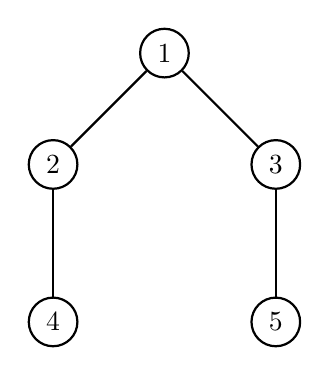
\begin{tikzpicture}[auto, node distance=2cm,
                    thick, main node/.style={circle, draw}]
    \node[main node] (1)                                {$1$};
    \node[main node] (2) [below left of=1]              {$2$};
    \node[main node] (3) [below right of=1]             {$3$};
    \node[main node] (4) [below of=2]                   {$4$};
    \node[main node] (5) [below of=3]                   {$5$};

    \path[every node/.style={}]
    (1) edge node {} (2)
        edge node {} (3)
    (2) edge node {} (4)
    (3) edge node {} (5);
\end{tikzpicture}
\qquad
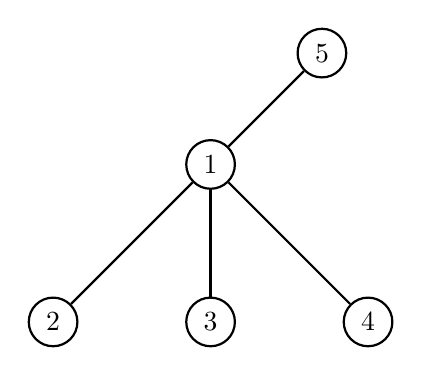
\begin{tikzpicture}[auto, node distance=2cm,
                    thick, main node/.style={circle, draw}]
    \node[main node] (1)                                {$1$};
    \node[main node] (5) [above right of=1]             {$5$};
    \node[main node] (2) [below of=1, xshift=-2cm]      {$2$};
    \node[main node] (3) [below of=1]                   {$3$};
    \node[main node] (4) [below of=1, xshift=2cm]       {$4$};

    \path[every node/.style={}]
    (5) edge node {} (1)
    (1) edge node {} (2)
        edge node {} (3)
        edge node {} (4);
\end{tikzpicture}
}
\end{figure}

上圖為範例測試資料一和二所給定的兩棵有根樹,左邊的樹以節點 \(1\)
為根、右邊的樹以節點 \(5\) 為根。以節點對 \(\{2, 5\}\)
為例,我們可知在左樹 \(\textrm{lca}(2, 5)=1\),節點 \(5\) 移動到節點
\(1\) 需要兩步,但節點 \(2\) 移動到節點 \(1\)
只需要一步,因此他們在左樹的祖先關係距離為 \(1\)。注意到因為節點對
\(\{2, 5\}\) 在右樹互為祖先關係,當 \(k=0\) 時,節點對 \(\{2, 5\}\)
會被視為有差異的節點對,同理,節點對 \(\{2, 4\}\) 以及 \(\{4, 5\}\)
都是有差異的節點對,因此,上圖中的兩棵樹在 \(k=0\) 時的距離函數值為
\(3\);而當 \(k=1\) 時,只有 \(\{4, 5\}\) 因在左樹的祖先關係距離為 \(2\)
會被視為有差異的節點對,距離函數值僅為 \(1\)。

請你撰寫一支程式,幫助小明和小花計算給定的兩棵有根樹在誤差參數為 \(k\)
時的距離函數值。

\subsection{輸入格式}

\begin{format}
\f{
$n$ $k$
$p_1$ $p_2$ $\cdots$ $p_n$
$q_1$ $q_2$ $\cdots$ $q_n$
}
\end{format}

\begin{itemize}
\tightlist
\item
  \(n\) 代表給定的樹之大小。
\item
  \(k\) 代表這次量測兩棵樹距離時使用的誤差參數。
\item
  在給定的第一棵樹中,節點 \(i\) 的父節點為 \(p_i\)。特別地,當
  \(p_i = 0\) 時,表示節點 \(i\) 是第一棵樹的根節點。
\item
  在給定的第二棵樹中,節點 \(i\) 的父節點為 \(q_i\)。特別地,當
  \(q_i = 0\) 時,表示節點 \(i\) 是第二棵樹的根節點。
\end{itemize}

\subsection{輸出格式}

\begin{format}
\f{
$d$
}
\end{format}

\begin{itemize}
\tightlist
\item
  \(d\) 為一整數,代表給定的兩棵樹在誤差參數 \(k\) 時的距離函數值。
\end{itemize}

\subsection{測資限制}

\begin{itemize}
\tightlist
\item
  \(1 \le n \le 2\times 10^5\)。
\item
  \(0 \le k < n\)。
\item
  \(0 \le p_i, q_i \le n\)。
\item
  保證存在唯一一個 \(u\) 滿足 \(p_u = 0\),且序列 \(p\) 形成一個以 \(u\)
  為根的有根樹。
\item
  保證存在唯一一個 \(v\) 滿足 \(q_v = 0\),且序列 \(q\) 形成一個以 \(v\)
  為根的有根樹。
\item
  輸入的數皆為整數。
\end{itemize}

\subsection{範例測試}

\begin{example}
\exmp{
5 0
0 1 1 2 3
5 1 1 1 0
}{%
3
}%
\exmp{
5 1
0 1 1 2 3
5 1 1 1 0
}{%
1
}%
\exmp{
10 0
6 5 5 5 0 3 4 6 6 6
6 4 5 7 10 7 10 7 3 0
}{%
22
}%
\exmp{
10 2
0 1 2 3 4 5 6 7 8 9
8 7 6 5 0 5 4 3 2 1
}{%
6
}%
\end{example}

\subsection{評分說明}

本題共有五組子任務,條件限制如下所示。
每一組可有一或多筆測試資料,該組所有測試資料皆需答對才會獲得該組分數。

\begin{longtable}[]{@{}ccl@{}}
\toprule
子任務 & 分數 & 額外輸入限制 \\
\midrule
\endhead
1 & \(4\) & \(n \le 100\)。 \\
2 & \(10\) & \(n \le 3000\)。 \\
3 & \(32\) & \(k = 0\)。 \\
4 & \(25\) & \(k \le 20\)。 \\
5 & \(29\) & 無額外限制。 \\
\bottomrule
\end{longtable}

\section{棲息地分配 (habitat distribution)}

\subsection{問題描述}

有 \(n\) 隻貓活動於某個地區,每隻貓各有其棲息地,編號為 \(1\) 到
\(n\)。棲息地之間有 \(m\) 條道路連接,道路總數不超過 \(2n-4\)。第 \(i\)
條道路連接第 \(a_i\) 個棲息地和第 \(b_i\)
個棲息地,貓可以沿著這些道路在棲息地之間\textbf{雙向}移動,且不會有兩條不同的道路連接著同一對棲息地。有
\(3\) 個動保團體要接管此地區,請你協助將這 \(n\) 個棲息地分配給這 \(3\)
個團體,滿足以下要求:

\begin{itemize}
\tightlist
\item
  每個棲息地僅由 \(1\) 個團體管理,且每個團體需要管理至少 \(1\)
  個棲息地。每個團體所屬的棲息地之間不一定要連通。
\item
  為了方便管理,每個團體會移除由該團體負責的棲息地之間的道路。換句話說,若有一條道路連接的兩個棲息地被分配到同一個團體,該道路會被移除。
\item
  這些道路移除後,剩餘的道路不可以形成「環」,以免貓可能會繞著環奔跑,讓工作人員難以捉捕。也就是說,不可以存在一個兩兩相異的棲息地序列
  \(v_1,v_2,\ldots, v_k\)\hspace{0pt},滿足 \(k \ge 3\),且對於所有
  \(1\le i < k\),棲息地 \(v_i\)\hspace{0pt} 和棲息地
  \(v_{i+1}\)\hspace{0pt} 都有一條未被移除的道路連接、同時
  \(v_k\)\hspace{0pt} 和 \(v_1\)\hspace{0pt}
  也有一條未被移除的道路連接。
\end{itemize}

舉例,有 \(5\) 個棲息地,道路連接如下圖所示

\begin{center}
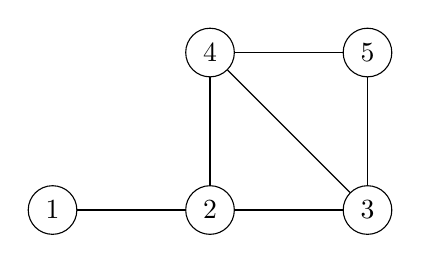
\begin{tikzpicture}
  % Define nodes
  \node[draw, circle] (a) at (0,0) {$1$};
  \node[draw, circle] (b) at (2,0) {$2$};
  \node[draw, circle] (c) at (4,0) {$3$};
  \node[draw, circle] (d) at (2,2) {$4$};
  \node[draw, circle] (e) at (4,2) {$5$};

  % Draw edges
  \draw (a) -- (b);
  \draw (b) -- (c);
  \draw (c) -- (d);
  \draw (d) -- (e);
  \draw (e) -- (c);
  \draw (d) -- (b);
\end{tikzpicture}
\end{center}

我們可以將第 \(3\), \(4\), \(5\) 個棲息地分配給第 \(1\) 個團體,第 \(1\)
個棲息地分配給第 \(2\) 個團體,第 \(2\) 個棲息地分配給第 \(3\) 個團體。
移除掉道路後,如下圖所示

\begin{center}
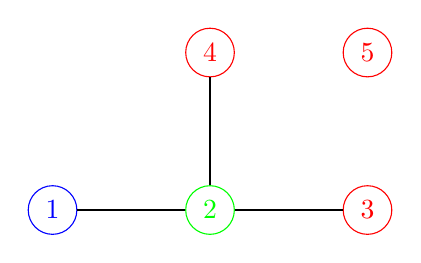
\begin{tikzpicture}
  % Define nodes
  \node[draw, circle, blue] (a) at (0,0) {$1$};
  \node[draw, circle, green] (b) at (2,0) {$2$};
  \node[draw, circle, red] (c) at (4,0) {$3$};
  \node[draw, circle, red] (d) at (2,2) {$4$};
  \node[draw, circle, red] (e) at (4,2) {$5$};

  % Draw edges
  \draw (a) -- (b);
  \draw (b) -- (c);
  \draw (d) -- (b);
\end{tikzpicture}
\end{center}

剩餘道路不存在環,所以這是一種滿足目標的分配方式。

請輸出這 \(3\)
個團體應該分別管理哪些棲息地,若有多種分配方式滿足條件,輸出任意一種。

\subsection{輸入格式}

輸入包含多筆測試資料

\begin{format}
\f{
$t$
$test_1$
$test_2$
$\vdots$
$test_t$
}
\end{format}

\begin{itemize}
\tightlist
\item
  \(t\) 表示測試資料個數。
\item
  \(test_i\) 為第\(i\)筆測試資料。
\end{itemize}

每一筆測試資料的輸入格式如下

\begin{format}
\f{
$n$ $m$
$a_1$ $b_1$
$a_2$ $b_2$
$\vdots$
$a_m$ $b_m$
}
\end{format}

\begin{itemize}
\tightlist
\item
  \(n\) 為貓的棲息地數量。
\item
  \(m\) 為道路數量。
\item
  \(a_i\), \(b_i\)
  為第\(i\)條道路連接的棲息地編號。不會有兩條不同的道路連接著同一對棲息地。
\end{itemize}

\subsection{輸出格式}

輸出 \(t\) 筆測試資料之答案

\begin{format}
\f{
$answer_1$
$answer_2$
$\vdots$
$answer_t$
}
\end{format}

\begin{itemize}
\tightlist
\item
  \(answer_i\) 為第\(i\)筆測試資料之答案。
\end{itemize}

每一筆測試資料答案的輸出格式如下

\begin{format}
\f{
$k_1$ $c_{1,1}$ $\cdots$ $c_{1,k_1}$
$k_2$ $c_{2,1}$ $\cdots$ $c_{1,k_2}$
$k_3$ $c_{3,1}$ $\cdots$ $c_{1,k_3}$
}
\end{format}

\begin{itemize}
\tightlist
\item
  \(k_i\) 為第\(i\)個團體分配到的棲息地總數。
\item
  \(c_{i,j}\) 為第\(i\)個團體分配到的第\(j\)個棲息地。
\end{itemize}

若該筆測試資料不存在所求的分法,請輸出 -1

\begin{format}
\f{
-1
}
\end{format}

\subsection{測資限制}

\begin{itemize}
\tightlist
\item
  \(1 \le t \le 3\times 10^5\)。
\item
  \(3 \le n \le 3\times 10^5\)。
\item
  \(0 \le m \le 2n - 4\)。
\item
  \(1 \le a_i, b_i \le n\),\(a_i \neq b_i\)。
\item
  所有測試資料中,\(n\) 的總和不超過 \(3\times 10^5\)。
\end{itemize}

\subsection{範例測試}

\begin{example}
\exmp{
1
5 6
1 2
2 3
3 4
4 5
5 3
4 2
}{%
3 3 4 5
1 1
1 2
}%
\exmp{
2
5 4
1 2
1 3
3 4
3 5
5 4
1 2
2 3
1 3
4 5
}{%
2 1 2
1 3
2 4 5
3 1 2 3
1 4
1 5
}%
\end{example}

\subsection{評分說明}

本題共有四組子任務,條件限制如下所示。
每一組可有一或多筆測試資料,該組所有測試資料皆需答對才會獲得該組分數。

\begin{longtable}[]{@{}ccl@{}}
\toprule
子任務 & 分數 & 額外輸入限制 \\
\midrule
\endhead
1 & \(3\) & 輸入滿足 \(m = n - 1\),且所有的棲息地連通。 \\
2 & \(23\) & 輸入保證存在兩個以上的棲息地互相無法抵達。 \\
3 & \(28\) & 輸入滿足所有測試資料中,\(n\) 的總和不超過 \(500\)。 \\
4 & \(46\) & 無額外限制。 \\
\bottomrule
\end{longtable}
